\chapter{Resultados Experimentais}
\label{cap:results}

Neste capítulo vamos apresentar alguns testes feitos para verificar o desempenho de um cliente escrito utilizando a biblioteca http2 quando submetido a diferentes fluxos de dados. Para efeito de análise, vamos utilizá-la para criar um cliente HTTP/2, chamado http2, a fim de compará-lo com outros clientes escritos em suas respectivas bibliotecas que também implementam o lado cliente do protocolo HTTP/2.

Os testes foram conduzidos da seguinte forma: selecionamos três clientes HTTP/2 populares para realizarem 10 requisições para um mesmo servidor HTTP/2 e para processarem as respostas enviadas por esse servidor simultaneamente na mesma conexão TCP. Essas 10 requisições serão feitas 10 vezes seguidas através de 10 diferentes execuções do cliente em particular. O servidor escolhido foi o servidor nghttpd da biblioteca nghttp2 (versão 1.30.0) \cite{nghttp2}. Os clientes escolhidos foram:

\begin{itemize}
    \item o cliente da biblioteca nghttp2 (versão 1.30.0): nghttp \cite{nghttp2}.
    \item um cliente que utiliza a biblioteca ``lua-http'' de Lua (versão 0.2) \cite{DaurminatorLuaHTTP}: lua-http.
    \item um cliente que utiliza a biblioteca ``http2'' de Node.js (versão 8.10.0) \cite{Nodejs}: nodejs.
\end{itemize}

O computador que hospedou o cliente HTTP/2 tem como especificações técnicas um processador Intel Core i3-4340 com 4 núcleos, cada um com 3.6 GHz; 6 GB de memória RAM; Ethernet 100 Mb/s e executa o sistema operacional GNU/Linux de 64 bits, {\em kernel} 4.4.0-17134-Microsoft. O computador que hospedou o servidor HTTP/2 tem como especificações técnicas um processador AMD Dual Core E1-500 com 2 núcleos, cada um com 1.48 GHz; 4 GB de memória RAM; Ethernet 100 Mb/s e  executa o sistema operacional GNU/Linux de 64 bits, {\em kernel} 4.15.0-38-generic.

Tentamos diversificar a escolha dos clientes de modo a testarmos como diferentes métodos para implementá-los podem impactar em seus desempenhos nos cenários de teste deste trabalho. O cliente nghttp foi escolhido por ter sido implementado na linguagem compilada C, na qual a expectativa é que ele obtenha um desempenho superior em relação aos demais, que são implementados em linguagens de {\em scripting}. O cliente lua-http foi selecionado por se assemelhar com o cliente http2 em termos da linguagem Lua, apesar de ambos empregarem diferentes mecanismos de implementação. O cliente nodejs foi escolhido por também ter sido implementado em uma linguagem de {\em scripting}.

Durante a execução dos testes, conectamos o computador cliente e o computador servidor na mesma rede LAN, bem como suspendemos quaisquer intervenções externas da rede que possam impactar negativamente a vazão de dados nos enlaces Ethernet. Apesar de estudos como \cite{Saxce7179400, Oda8319285} mostrarem que o HTTP/2 apenas traz vantagens em certas condições de rede, é importante conduzir testes para comparar o desempenho da implementação do cliente http2 com outros clientes HTTP/2 quando múltiplas requisições simultâneas são feitas na mesma conexão TCP, ao mesmo tempo evitando uma fuga ao escopo deste trabalho.

Nas Figuras \ref{fig:1,5MB}, \ref{fig:10MB} e \ref{fig:100MB}, medimos o tempo médio de execução de três testes feitos como descritos a seguir. Em cada teste, realizamos 10 execuções de cada cliente, cada execução submetendo um total de 10 requisições simultâneas na mesma conexão TCP (e não sequenciais ou em diferentes conexões TCP para cada requisição, como no HTTP/1.1) para o servidor.

O primeiro retrata melhor o cenário atual de uma requisição por uma página Web de tamanho típico de 1,5 megabytes \cite{HTTPArchive}. Pelos resultados mostrados na Figura \ref{fig:1,5MB}, observamos que o cliente da biblioteca http2 se sobressaiu no cenário de uma curta troca de dados e, nesse caso, com tempo de 1,08 segundos para baixar 1 megabyte. Em comparação, para baixar 1 megabyte, o cliente lua-http precisou de 1,13 segundos; o cliente nodejs, 1,38 segundos e o nghttp, 1,1 segundos.

O segundo teste fez com que os clientes realizassem requisições para um arquivo de 10 MB. Pelos registros resumidos na Figura \ref{fig:10MB}, o cliente http2 em questão ainda mostra uma boa vazão ao levar 1,11 segundos para baixar 1 megabyte nessa situação de um médio fluxo de dados. Em comparação, para baixar 1 megabyte, o cliente lua-http precisou de 1,13 segundos; o cliente nodejs, 1,17 segundos e o cliente nghttp, 1,10 segundos.

No último teste, os clientes submeteram requisições para um arquivo de 100 MB. Depois, medimos o tempo médio de execução (em segundos) e obtivemos o satisfatório resultado de que o cliente http2 teve um tempo comparável com cliente nghttp. Em média, para baixar 1 megabyte nesse cenário, o cliente http2 levou 0,89 segundos. Em comparação, para baixar 1 megabyte, o cliente lua-http precisou de 0,94 segundos; o cliente nodejs, 0,89 segundos e o cliente nghttp, também 0,89 segundos.

É importante observar que o cliente http2 foi implementado visando funcionalidades mínimas necessárias para um cliente HTTP/2, pois ela somente cumpre com os requisitos mínimos do protocolo HTTP/2. Em contrapartida, as outras implementações, por serem mais maduras, podem ter uma lógica de processamento mais bem elaborada internamente, podendo impactar mais na vazão dos dados transmitidos pelo servidor.

\begin{figure}[hbt!]
 \centering
  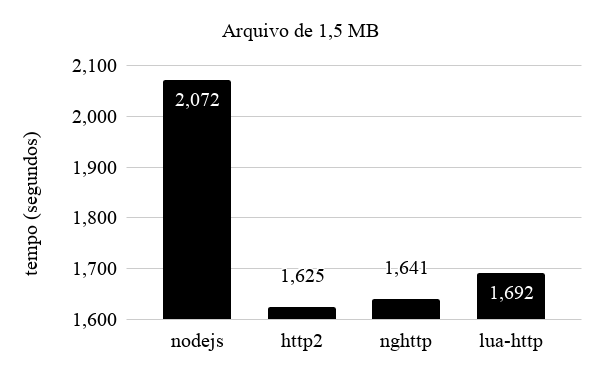
\includegraphics[width=0.65\textwidth]{./fig/1,5MB}
 \caption{Tempo médio de execução de quatro clientes HTTP/2, onde cada um fez 10 requisições de um arquivo de 1,5 megabytes.}
 \label{fig:1,5MB}
\end{figure}

\begin{figure}[hbt!]
 \centering
  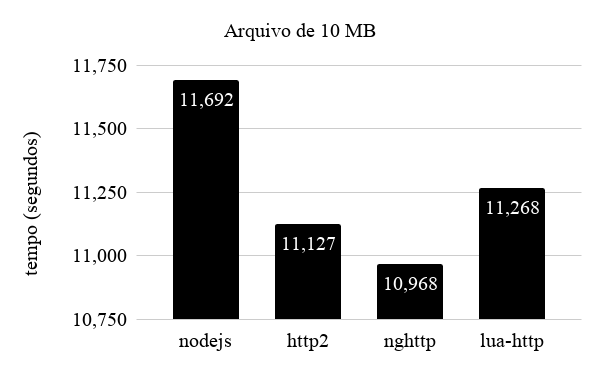
\includegraphics[width=0.65\textwidth]{./fig/10MB}
 \caption{Tempo médio de execução de quatro clientes HTTP/2, onde cada um fez 10 requisições de um arquivo de 10 megabytes.}
 \label{fig:10MB}
\end{figure}

\begin{figure}[hbt!]
 \centering
  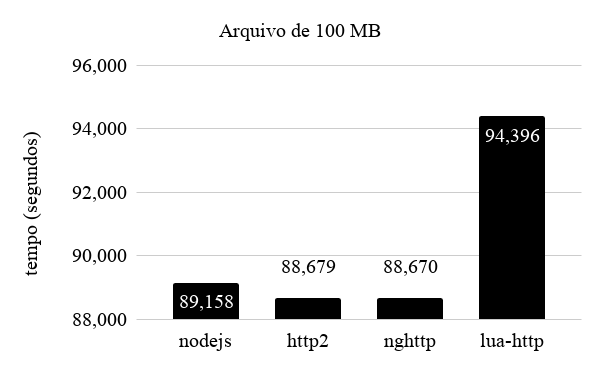
\includegraphics[width=0.65\textwidth]{./fig/100MB}
 \caption{Tempo médio de execução de quatro clientes HTTP/2, onde cada um fez 10 requisições de um arquivo de 100 megabytes.}
 \label{fig:100MB}
\end{figure}